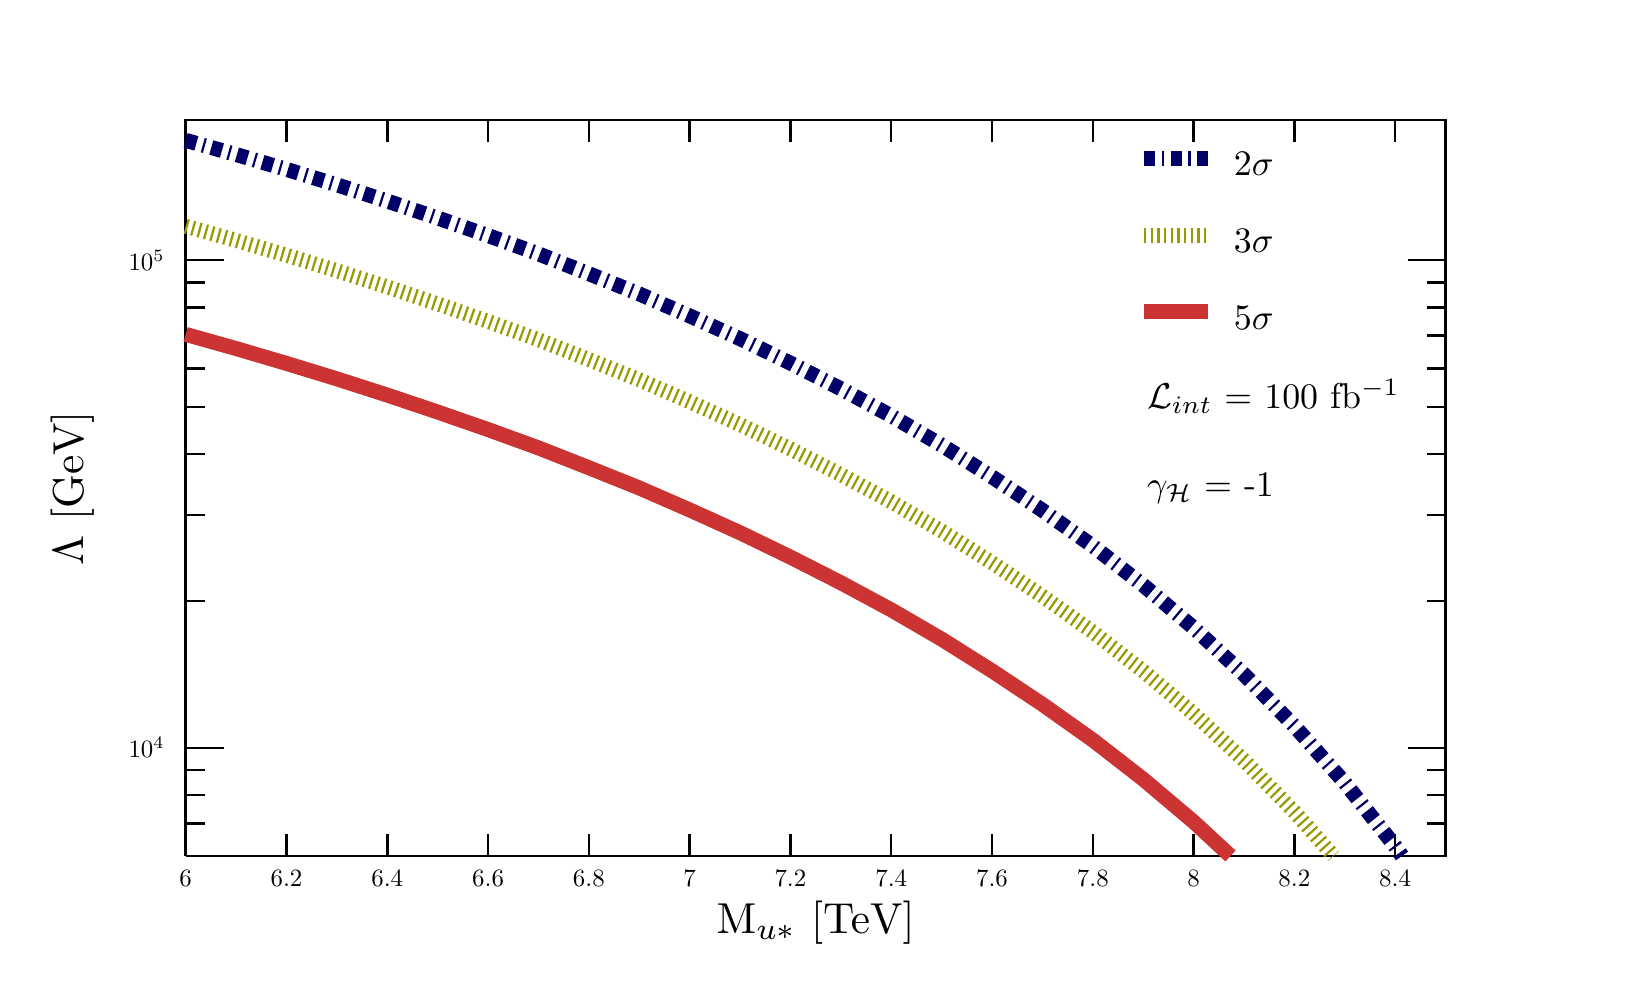
\begin{tikzpicture}
\pgfdeclareplotmark{cross} {
\pgfpathmoveto{\pgfpoint{-0.3\pgfplotmarksize}{\pgfplotmarksize}}
\pgfpathlineto{\pgfpoint{+0.3\pgfplotmarksize}{\pgfplotmarksize}}
\pgfpathlineto{\pgfpoint{+0.3\pgfplotmarksize}{0.3\pgfplotmarksize}}
\pgfpathlineto{\pgfpoint{+1\pgfplotmarksize}{0.3\pgfplotmarksize}}
\pgfpathlineto{\pgfpoint{+1\pgfplotmarksize}{-0.3\pgfplotmarksize}}
\pgfpathlineto{\pgfpoint{+0.3\pgfplotmarksize}{-0.3\pgfplotmarksize}}
\pgfpathlineto{\pgfpoint{+0.3\pgfplotmarksize}{-1.\pgfplotmarksize}}
\pgfpathlineto{\pgfpoint{-0.3\pgfplotmarksize}{-1.\pgfplotmarksize}}
\pgfpathlineto{\pgfpoint{-0.3\pgfplotmarksize}{-0.3\pgfplotmarksize}}
\pgfpathlineto{\pgfpoint{-1.\pgfplotmarksize}{-0.3\pgfplotmarksize}}
\pgfpathlineto{\pgfpoint{-1.\pgfplotmarksize}{0.3\pgfplotmarksize}}
\pgfpathlineto{\pgfpoint{-0.3\pgfplotmarksize}{0.3\pgfplotmarksize}}
\pgfpathclose
\pgfusepathqstroke
}
\pgfdeclareplotmark{cross*} {
\pgfpathmoveto{\pgfpoint{-0.3\pgfplotmarksize}{\pgfplotmarksize}}
\pgfpathlineto{\pgfpoint{+0.3\pgfplotmarksize}{\pgfplotmarksize}}
\pgfpathlineto{\pgfpoint{+0.3\pgfplotmarksize}{0.3\pgfplotmarksize}}
\pgfpathlineto{\pgfpoint{+1\pgfplotmarksize}{0.3\pgfplotmarksize}}
\pgfpathlineto{\pgfpoint{+1\pgfplotmarksize}{-0.3\pgfplotmarksize}}
\pgfpathlineto{\pgfpoint{+0.3\pgfplotmarksize}{-0.3\pgfplotmarksize}}
\pgfpathlineto{\pgfpoint{+0.3\pgfplotmarksize}{-1.\pgfplotmarksize}}
\pgfpathlineto{\pgfpoint{-0.3\pgfplotmarksize}{-1.\pgfplotmarksize}}
\pgfpathlineto{\pgfpoint{-0.3\pgfplotmarksize}{-0.3\pgfplotmarksize}}
\pgfpathlineto{\pgfpoint{-1.\pgfplotmarksize}{-0.3\pgfplotmarksize}}
\pgfpathlineto{\pgfpoint{-1.\pgfplotmarksize}{0.3\pgfplotmarksize}}
\pgfpathlineto{\pgfpoint{-0.3\pgfplotmarksize}{0.3\pgfplotmarksize}}
\pgfpathclose
\pgfusepathqfillstroke
}
\pgfdeclareplotmark{newstar} {
\pgfpathmoveto{\pgfqpoint{0pt}{\pgfplotmarksize}}
\pgfpathlineto{\pgfqpointpolar{44}{0.5\pgfplotmarksize}}
\pgfpathlineto{\pgfqpointpolar{18}{\pgfplotmarksize}}
\pgfpathlineto{\pgfqpointpolar{-20}{0.5\pgfplotmarksize}}
\pgfpathlineto{\pgfqpointpolar{-54}{\pgfplotmarksize}}
\pgfpathlineto{\pgfqpointpolar{-90}{0.5\pgfplotmarksize}}
\pgfpathlineto{\pgfqpointpolar{234}{\pgfplotmarksize}}
\pgfpathlineto{\pgfqpointpolar{198}{0.5\pgfplotmarksize}}
\pgfpathlineto{\pgfqpointpolar{162}{\pgfplotmarksize}}
\pgfpathlineto{\pgfqpointpolar{134}{0.5\pgfplotmarksize}}
\pgfpathclose
\pgfusepathqstroke
}
\pgfdeclareplotmark{newstar*} {
\pgfpathmoveto{\pgfqpoint{0pt}{\pgfplotmarksize}}
\pgfpathlineto{\pgfqpointpolar{44}{0.5\pgfplotmarksize}}
\pgfpathlineto{\pgfqpointpolar{18}{\pgfplotmarksize}}
\pgfpathlineto{\pgfqpointpolar{-20}{0.5\pgfplotmarksize}}
\pgfpathlineto{\pgfqpointpolar{-54}{\pgfplotmarksize}}
\pgfpathlineto{\pgfqpointpolar{-90}{0.5\pgfplotmarksize}}
\pgfpathlineto{\pgfqpointpolar{234}{\pgfplotmarksize}}
\pgfpathlineto{\pgfqpointpolar{198}{0.5\pgfplotmarksize}}
\pgfpathlineto{\pgfqpointpolar{162}{\pgfplotmarksize}}
\pgfpathlineto{\pgfqpointpolar{134}{0.5\pgfplotmarksize}}
\pgfpathclose
\pgfusepathqfillstroke
}
\definecolor{c}{rgb}{1,1,1};
\draw [color=c, fill=c] (0,0) rectangle (20,11.6806);
\draw [color=c, fill=c] (2,1.16806) rectangle (18,10.5125);
\definecolor{c}{rgb}{0,0,0};
\draw [c,line width=0.9] (2,1.16806) -- (2,10.5125) -- (18,10.5125) -- (18,1.16806) -- (2,1.16806);
\definecolor{c}{rgb}{1,1,1};
\draw [color=c, fill=c] (2,1.16806) rectangle (18,10.5125);
\definecolor{c}{rgb}{0,0,0};
\draw [c,line width=0.9] (2,1.16806) -- (2,10.5125) -- (18,10.5125) -- (18,1.16806) -- (2,1.16806);
\draw [c,line width=0.9] (2,1.16806) -- (18,1.16806);
\draw (10,0.327056) node[scale=1.56475, color=c, rotate=0]{M$_{u*}$ [TeV]};
\draw [c,line width=0.9] (2,1.44839) -- (2,1.16806);
\draw [c,line width=0.9] (3.28,1.44839) -- (3.28,1.16806);
\draw [c,line width=0.9] (4.56,1.44839) -- (4.56,1.16806);
\draw [c,line width=0.9] (5.84,1.44839) -- (5.84,1.16806);
\draw [c,line width=0.9] (7.12,1.44839) -- (7.12,1.16806);
\draw [c,line width=0.9] (8.4,1.44839) -- (8.4,1.16806);
\draw [c,line width=0.9] (9.68,1.44839) -- (9.68,1.16806);
\draw [c,line width=0.9] (10.96,1.44839) -- (10.96,1.16806);
\draw [c,line width=0.9] (12.24,1.44839) -- (12.24,1.16806);
\draw [c,line width=0.9] (13.52,1.44839) -- (13.52,1.16806);
\draw [c,line width=0.9] (14.8,1.44839) -- (14.8,1.16806);
\draw [c,line width=0.9] (16.08,1.44839) -- (16.08,1.16806);
\draw [c,line width=0.9] (17.36,1.44839) -- (17.36,1.16806);
\draw [c,line width=0.9] (17.36,1.44839) -- (17.36,1.16806);
\draw [anchor=base] (2,0.782598) node[scale=0.900036, color=c, rotate=0]{6};
\draw [anchor=base] (3.28,0.782598) node[scale=0.900036, color=c, rotate=0]{6.2};
\draw [anchor=base] (4.56,0.782598) node[scale=0.900036, color=c, rotate=0]{6.4};
\draw [anchor=base] (5.84,0.782598) node[scale=0.900036, color=c, rotate=0]{6.6};
\draw [anchor=base] (7.12,0.782598) node[scale=0.900036, color=c, rotate=0]{6.8};
\draw [anchor=base] (8.4,0.782598) node[scale=0.900036, color=c, rotate=0]{7};
\draw [anchor=base] (9.68,0.782598) node[scale=0.900036, color=c, rotate=0]{7.2};
\draw [anchor=base] (10.96,0.782598) node[scale=0.900036, color=c, rotate=0]{7.4};
\draw [anchor=base] (12.24,0.782598) node[scale=0.900036, color=c, rotate=0]{7.6};
\draw [anchor=base] (13.52,0.782598) node[scale=0.900036, color=c, rotate=0]{7.8};
\draw [anchor=base] (14.8,0.782598) node[scale=0.900036, color=c, rotate=0]{8};
\draw [anchor=base] (16.08,0.782598) node[scale=0.900036, color=c, rotate=0]{8.2};
\draw [anchor=base] (17.36,0.782598) node[scale=0.900036, color=c, rotate=0]{8.4};
\draw [c,line width=0.9] (2,10.5125) -- (18,10.5125);
\draw [c,line width=0.9] (2,10.2322) -- (2,10.5125);
\draw [c,line width=0.9] (3.28,10.2322) -- (3.28,10.5125);
\draw [c,line width=0.9] (4.56,10.2322) -- (4.56,10.5125);
\draw [c,line width=0.9] (5.84,10.2322) -- (5.84,10.5125);
\draw [c,line width=0.9] (7.12,10.2322) -- (7.12,10.5125);
\draw [c,line width=0.9] (8.4,10.2322) -- (8.4,10.5125);
\draw [c,line width=0.9] (9.68,10.2322) -- (9.68,10.5125);
\draw [c,line width=0.9] (10.96,10.2322) -- (10.96,10.5125);
\draw [c,line width=0.9] (12.24,10.2322) -- (12.24,10.5125);
\draw [c,line width=0.9] (13.52,10.2322) -- (13.52,10.5125);
\draw [c,line width=0.9] (14.8,10.2322) -- (14.8,10.5125);
\draw [c,line width=0.9] (16.08,10.2322) -- (16.08,10.5125);
\draw [c,line width=0.9] (17.36,10.2322) -- (17.36,10.5125);
\draw [c,line width=0.9] (17.36,10.2322) -- (17.36,10.5125);
\draw [c,line width=0.9] (2,1.16806) -- (2,10.5125);
\draw (0.56,5.84029) node[scale=1.56475, color=c, rotate=90]{$\Lambda$ [GeV]};
\draw [c,line width=0.9] (2.24,1.1685) -- (2,1.1685);
\draw [c,line width=0.9] (2.24,1.58303) -- (2,1.58303);
\draw [c,line width=0.9] (2.24,1.94212) -- (2,1.94212);
\draw [c,line width=0.9] (2.24,2.25886) -- (2,2.25886);
\draw [c,line width=0.9] (2.48,2.54219) -- (2,2.54219);
\draw [anchor= east] (1.844,2.54219) node[scale=0.900036, color=c, rotate=0]{$10^{4}$};
\draw [c,line width=0.9] (2.24,4.40617) -- (2,4.40617);
\draw [c,line width=0.9] (2.24,5.49653) -- (2,5.49653);
\draw [c,line width=0.9] (2.24,6.27015) -- (2,6.27015);
\draw [c,line width=0.9] (2.24,6.87022) -- (2,6.87022);
\draw [c,line width=0.9] (2.24,7.36051) -- (2,7.36051);
\draw [c,line width=0.9] (2.24,7.77504) -- (2,7.77504);
\draw [c,line width=0.9] (2.24,8.13413) -- (2,8.13413);
\draw [c,line width=0.9] (2.24,8.45087) -- (2,8.45087);
\draw [c,line width=0.9] (2.48,8.7342) -- (2,8.7342);
\draw [anchor= east] (1.844,8.7342) node[scale=0.900036, color=c, rotate=0]{$10^{5}$};
\draw [c,line width=0.9] (18,1.16806) -- (18,10.5125);
\draw [c,line width=0.9] (17.76,1.1685) -- (18,1.1685);
\draw [c,line width=0.9] (17.76,1.58303) -- (18,1.58303);
\draw [c,line width=0.9] (17.76,1.94212) -- (18,1.94212);
\draw [c,line width=0.9] (17.76,2.25886) -- (18,2.25886);
\draw [c,line width=0.9] (17.52,2.54219) -- (18,2.54219);
\draw [c,line width=0.9] (17.76,4.40617) -- (18,4.40617);
\draw [c,line width=0.9] (17.76,5.49653) -- (18,5.49653);
\draw [c,line width=0.9] (17.76,6.27015) -- (18,6.27015);
\draw [c,line width=0.9] (17.76,6.87022) -- (18,6.87022);
\draw [c,line width=0.9] (17.76,7.36051) -- (18,7.36051);
\draw [c,line width=0.9] (17.76,7.77504) -- (18,7.77504);
\draw [c,line width=0.9] (17.76,8.13413) -- (18,8.13413);
\draw [c,line width=0.9] (17.76,8.45087) -- (18,8.45087);
\draw [c,line width=0.9] (17.52,8.7342) -- (18,8.7342);
\definecolor{c}{rgb}{0,0,0.4};
\draw [c,dash pattern=on 4.00pt off 2.40pt on 0.80pt off 2.40pt ,line width=5.4] (2,10.2564) -- (2.64,10.0765) -- (3.28,9.88762) -- (3.92,9.69143) -- (4.56,9.48545) -- (5.2,9.27013) -- (5.84,9.04747) -- (6.48,8.81468) -- (7.12,8.56287) --
 (7.76,8.30609) -- (8.4,8.02684) -- (9.04,7.73741) -- (9.68,7.42743) -- (10.32,7.10208) -- (10.96,6.75777) -- (11.6,6.38578) -- (12.24,5.98315) -- (12.88,5.558) -- (13.52,5.10431) -- (14.16,4.60716) -- (14.8,4.06636) -- (15.44,3.47376) --
 (16.08,2.81852) -- (16.72,2.0988) -- (17.36,1.29108) -- (17.447,1.16806);
\definecolor{c}{rgb}{0.6,0.6,0};
\draw [c,dash pattern=on 0.80pt off 1.60pt ,line width=5.4] (2,9.16602) -- (2.64,8.9861) -- (3.28,8.79724) -- (3.92,8.60107) -- (4.56,8.3951) -- (5.2,8.17977) -- (5.84,7.95711) -- (6.48,7.72431) -- (7.12,7.47251) -- (7.76,7.21573) -- (8.4,6.93648) --
 (9.04,6.64705) -- (9.68,6.33707) -- (10.32,6.01172) -- (10.96,5.66741) -- (11.6,5.29542) -- (12.24,4.8928) -- (12.88,4.46764) -- (13.52,4.01395) -- (14.16,3.51681) -- (14.8,2.97601) -- (15.44,2.38339) -- (16.08,1.72816) -- (16.5781,1.16806);
\definecolor{c}{rgb}{0.8,0.2,0.2};
\draw [c,line width=5.4] (2,7.79232) -- (2.64,7.6124) -- (3.28,7.42356) -- (3.92,7.22738) -- (4.56,7.02141) -- (5.2,6.80608) -- (5.84,6.58342) -- (6.48,6.35063) -- (7.12,6.09882) -- (7.76,5.84204) -- (8.4,5.56279) -- (9.04,5.27337) -- (9.68,4.96338)
 -- (10.32,4.63803) -- (10.96,4.29372) -- (11.6,3.92174) -- (12.24,3.51911) -- (12.88,3.09394) -- (13.52,2.64026) -- (14.16,2.14312) -- (14.8,1.60231) -- (15.269,1.16806);
\definecolor{c}{rgb}{0,0,0};
\draw (10,11.301) node[scale=1.2177, color=c, rotate=0]{ };
\draw [anchor=base west] (15.15,9.80681) node[scale=1.29711, color=c, rotate=0]{$2\sigma$};
\definecolor{c}{rgb}{0,0,0.4};
\draw [c,dash pattern=on 4.00pt off 2.40pt on 0.80pt off 2.40pt ,line width=5.4] (14.1725,10.0258) -- (14.9775,10.0258);
\definecolor{c}{rgb}{0,0,0};
\draw [anchor=base west] (15.15,8.83343) node[scale=1.29711, color=c, rotate=0]{$3\sigma$};
\definecolor{c}{rgb}{0.6,0.6,0};
\draw [c,dash pattern=on 0.80pt off 1.60pt ,line width=5.4] (14.1725,9.05244) -- (14.9775,9.05244);
\definecolor{c}{rgb}{0,0,0};
\draw [anchor=base west] (15.15,7.86005) node[scale=1.29711, color=c, rotate=0]{$5\sigma$};
\definecolor{c}{rgb}{0.8,0.2,0.2};
\draw [c,line width=5.4] (14.1725,8.07906) -- (14.9775,8.07906);
\definecolor{c}{rgb}{0,0,0};
\draw [anchor= west] (14.05,7.00834) node[scale=1.29711, color=c, rotate=0]{$\mathcal{L}_{int}$ = 100 fb$^{-1}$};
\draw [anchor= west] (14.05,5.84029) node[scale=1.29711, color=c, rotate=0]{$\gamma_{\mathcal{H}}$ = -1};
\end{tikzpicture}
